\documentclass[tikz,border=10pt]{standalone}
% Scale s = 0.015066 cm/px, y flipped, centre (305,222) px
\begin{document}
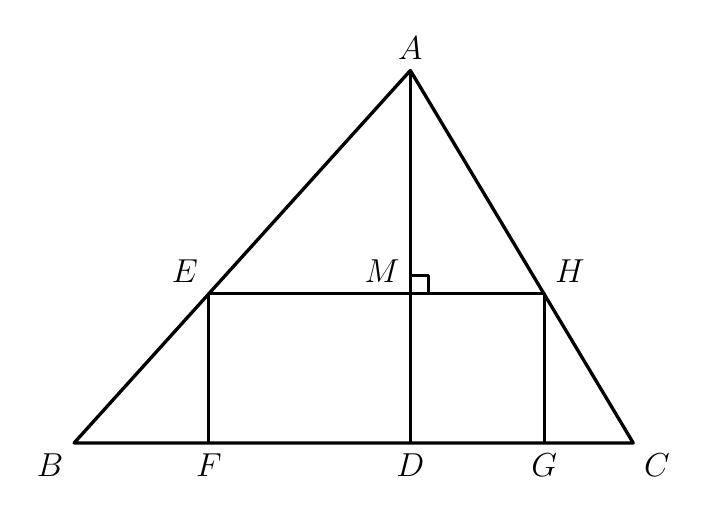
\begin{tikzpicture}[line width=1.2pt, line join=round]
  % Named points (converted from pixels)
  \coordinate (A) at (0.68,2.35);
  \coordinate (B) at (-3.59,-2.38);
  \coordinate (C) at (3.51,-2.38);
  \coordinate (D) at (0.68,-2.38);
  \coordinate (E) at (-1.88,-0.48);
  \coordinate (H) at (2.38,-0.48);
  \coordinate (M) at (0.68,-0.48);
  \coordinate (F) at (-1.88,-2.38);
  \coordinate (G) at (2.38,-2.38);

  % Triangle ABC
  \draw (A) -- (B) -- (C) -- cycle;
  % Altitude AD
  \draw (A) -- (D);
  % Chord EH
  \draw (E) -- (H);
  % Verticals EF and HG
  \draw (E) -- (F);
  \draw (H) -- (G);

  % Right-angle marker at M (between MA and MH), one mark only
  \draw (0.68,-0.25) -- (0.91,-0.25) -- (0.91,-0.48);

  % Labels
  \node[above, font=\fontsize{12}{14.4}\selectfont] at (A) {$A$};
  \node[below left, font=\fontsize{12}{14.4}\selectfont] at (B) {$B$};
  \node[below right, font=\fontsize{12}{14.4}\selectfont] at (C) {$C$};
  \node[below, font=\fontsize{12}{14.4}\selectfont] at (D) {$D$};
  \node[above left, font=\fontsize{12}{14.4}\selectfont] at (E) {$E$};
  \node[above right, font=\fontsize{12}{14.4}\selectfont] at (H) {$H$};
  \node[above left, font=\fontsize{12}{14.4}\selectfont] at (M) {$M$};
  \node[below, font=\fontsize{12}{14.4}\selectfont] at (F) {$F$};
  \node[below, font=\fontsize{12}{14.4}\selectfont] at (G) {$G$};
\end{tikzpicture}
\end{document}